\chapter{User Manual}
\label{chap:user}    

{\colorbox{red}{\textbf{NOTE:}}}\textbf{ Before you start working with the robot you have to attend a safety introduction. If you haven't got one yet, please contact your local robot administrator.}

The following user manual requires some basic knowledge about
\begin{itemize}
\item Linux/Ubuntu
\item Source code management with git
\item ROS usage
\end{itemize}
If you are missing some of this requirements or feel uncomfortable with what you are doing, please interrupt and ask somebody to help you before continuing.

\section{Hardware overview}
You can take a look of the technical data of Care-O-Bot on the official web site\footnote{\url{http://www.care-o-bot-research.org/care-o-bot-3/technical-data}} and \footnote{\url{http://www.care-o-bot-research.org/care-o-bot-3/components}}. Also you can see the distribution of the different Care-O-bots at \footnote{\url{http://www.ros.org/wiki/Robots/Care-O-bot/distribution}}.

An overview of the robot hardware is shown in the following picture.
\begin{center}
 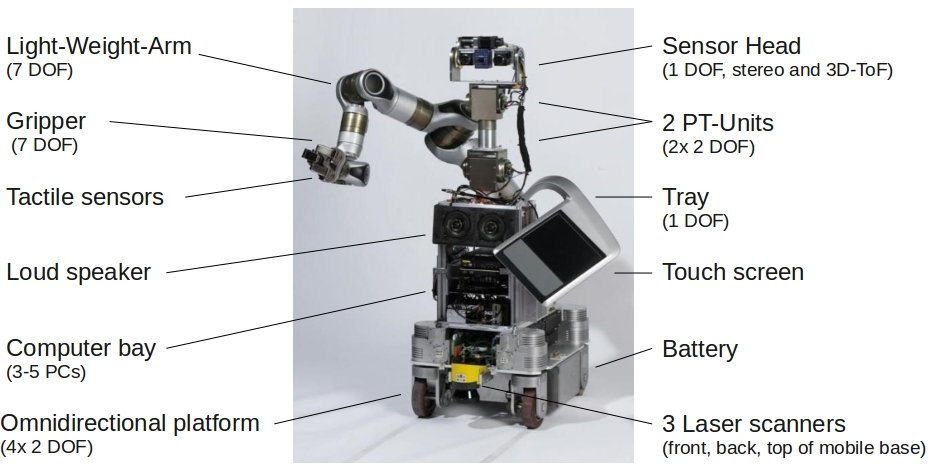
\includegraphics[width=0.95\textwidth]{images/hardware_overview.jpg}
\end{center}

\section{Software overview}\label{sec:software_overview}
We defined a layer called \textit{bringup layer}, which covers all hardware drivers and basic robot components. This is the layer where low level robot movements are enabled through the joystick or dashboard and the robot status including actuator and sensor information is acquired. In the following overview you can see the repositories which belong to the bringup layer.
\begin{itemize}
\item \texttt{cob\_extern}: The \texttt{cob\_extern} stack contains third party libraries needed for operating Care-O-bot. The packages are downloaded from the manufacturers website and not changed in any way.
\item \texttt{cob\_common}: The \texttt{cob\_common} stack hosts common packages that are used within the Care-O-bot repository. Also the urdf description of the robot, which is the kinematic and dynamic model of the robot, 3D models of robot components, information required for gazebo to simulate the COB and utility packages or common message and service definitions.
\item \texttt{schunk\_modular\_robotics}: This repository includes drivers and models for Schunk products, like powercubes or sdh.
\item \texttt{cob\_driver}: The cob\_driver stack includes packages that provide access to the Care-O-bot hardware through ROS messages, services and actions. E.g. for mobile base, arm, camera sensors, laser scanners, etc...
\item \texttt{cob\_command\_tools}: This stack provides the source code of the tools that you need to command the robot: \texttt{cob\_command\_gui}, \texttt{cob\_dashboard}, \texttt{cob\_script\_server} and \texttt{cob\_teleop}.
\item \texttt{cob\_robots}:  The \texttt{cob\_robots} stack collects Care-O-bot components that are used in bringing up a robot. The user's interface to the \texttt{cob\_robots} stack is \texttt{cob\_bringup}. In this package you find all the hardware configuration and launch files to bringup the hardware.
\item \texttt{cob\_environments}: This stack provides the parameters for default environment configurations.
\end{itemize}

\section{Batteries and power supply}
Care-O-bot is powered by a 48V battery, which can be a Gaia rechargeable Li ion battery (60 Ah 48V) or a plumb battery. The batteries can be charged with a maximum of 56V at 10A. The robot can be plugged in during operation.

\section{Emergency stop}\label{sec:emergency_stop}
Please be aware that not all robot movements are safe for you as an user, the robot itself and the environment. Therefore please don't hesitate to activate the emergency stop in situations which are not foreseen by the user. There are three ways of stopping the robot: On the robot you have two red buttons on the laterals, you can step into the safety fields of the Sick S300 scanners or you use the wireless emergency stop. Remember to recover the robot components with the command\_gui after an emergency stop was activated, check the status of the components using the dashboard.

\subsection{Emergency stop buttons}
Press the red buttons on the left and right side of the torso. To release the emergency stop, turn the buttons so that they come out again. After that turn the key to position II until you hear a "click".

\begin{center}
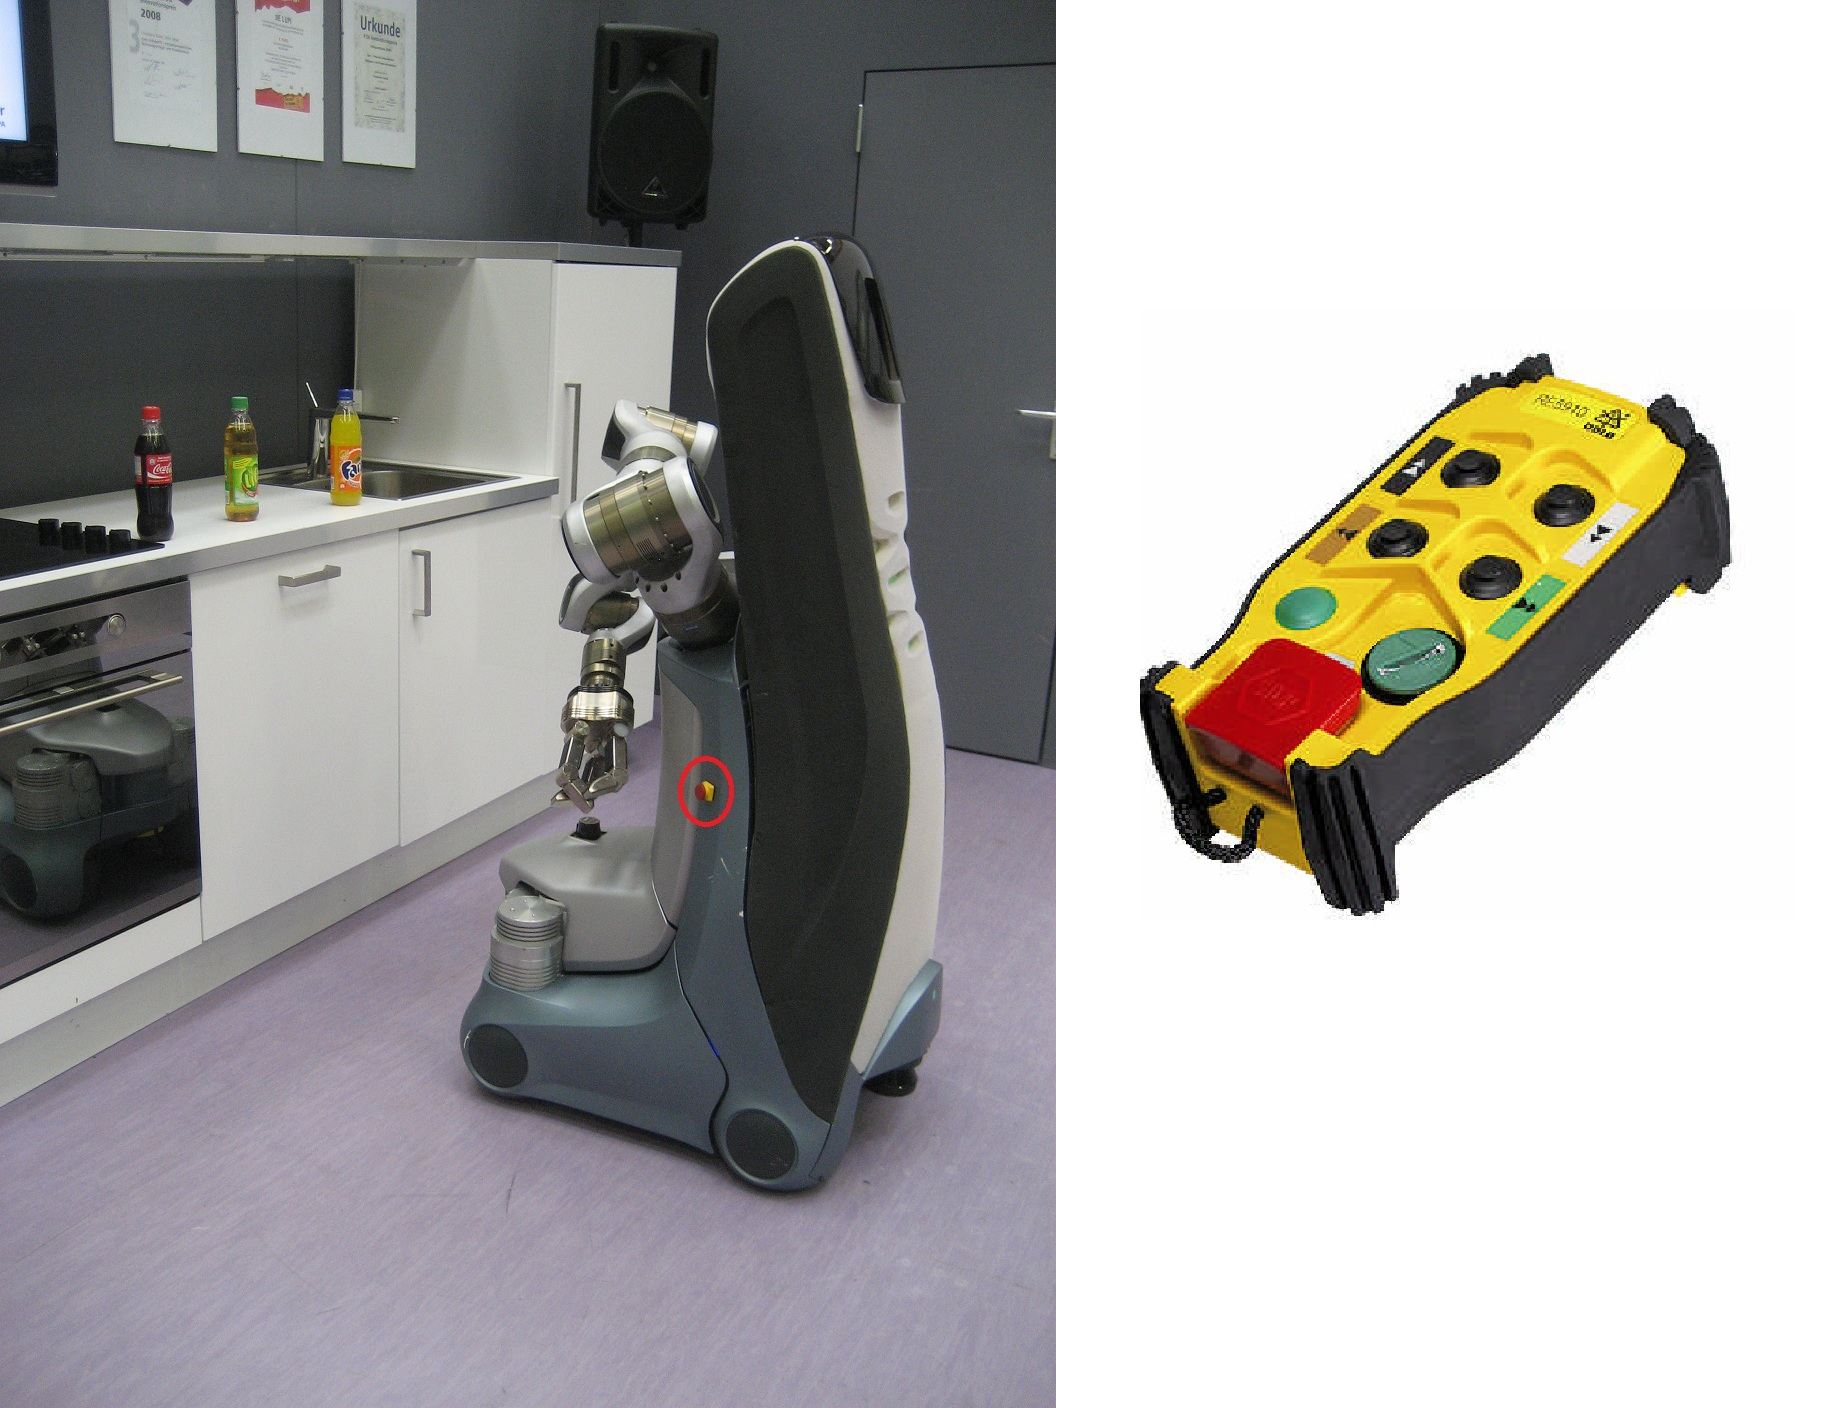
\includegraphics[width=0.65\textwidth]{images/em_stop.jpg}
\end{center}

\subsection{Safety field from the Sick S300 scanners}
If you step into the safety fields of the laser scanners the emergency stop is activated automatically. After the safety fields are free from any obstacle again the emergency stop is released on its own after a few seconds.

\begin{center}
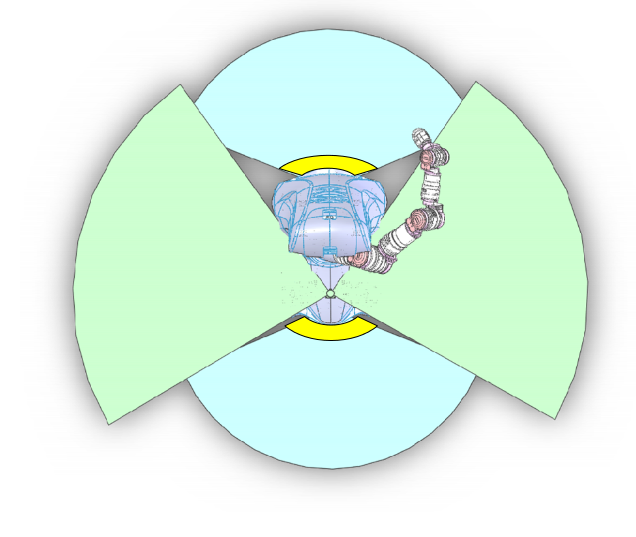
\includegraphics[width=0.65\textwidth]{images/protection_areas.png}
\end{center}

\subsection{Remote emergency stop control}
You can press the red button to stop the robot. To release the emergency stop you have to lift the red button and afterwards press the green button.


\textbf{NOTE}: If you hear a "click" while releasing the emergency stop, but the dashboard and command\_gui still show that the emergency stop is activated, turn the key to position II again and hold it for some seconds until the dashboard or command\_gui show no more emergency stop.


\section{Running the robot}
First you have to connect the power supply to the robot or you can use the battery pressing the battery button on the base. To switch the robot on you have to use the key. If you move it to position II and hold for a few seconds the robot will turn on. To turn of the robot turn the key to position I. 

After starting up the robot the emergency stop circuit is still activated. To enable power for the motors, keep the safety area of the Sick S300 scanners free of any obstacle and release the emergency buttons. In the case that the wireless emergency stop is active, release it by releasing the red button and pressing the green button afterwards. You should hear a "click" as soon as the emergency stop is released.

For safety reasons if the robot is not supervised any more, e.g. during a break, the emergency stop has to be activated. Never operate the robot without a local person supervising it being aware of the safety instructions (see separate safety instructions).

\begin{center}
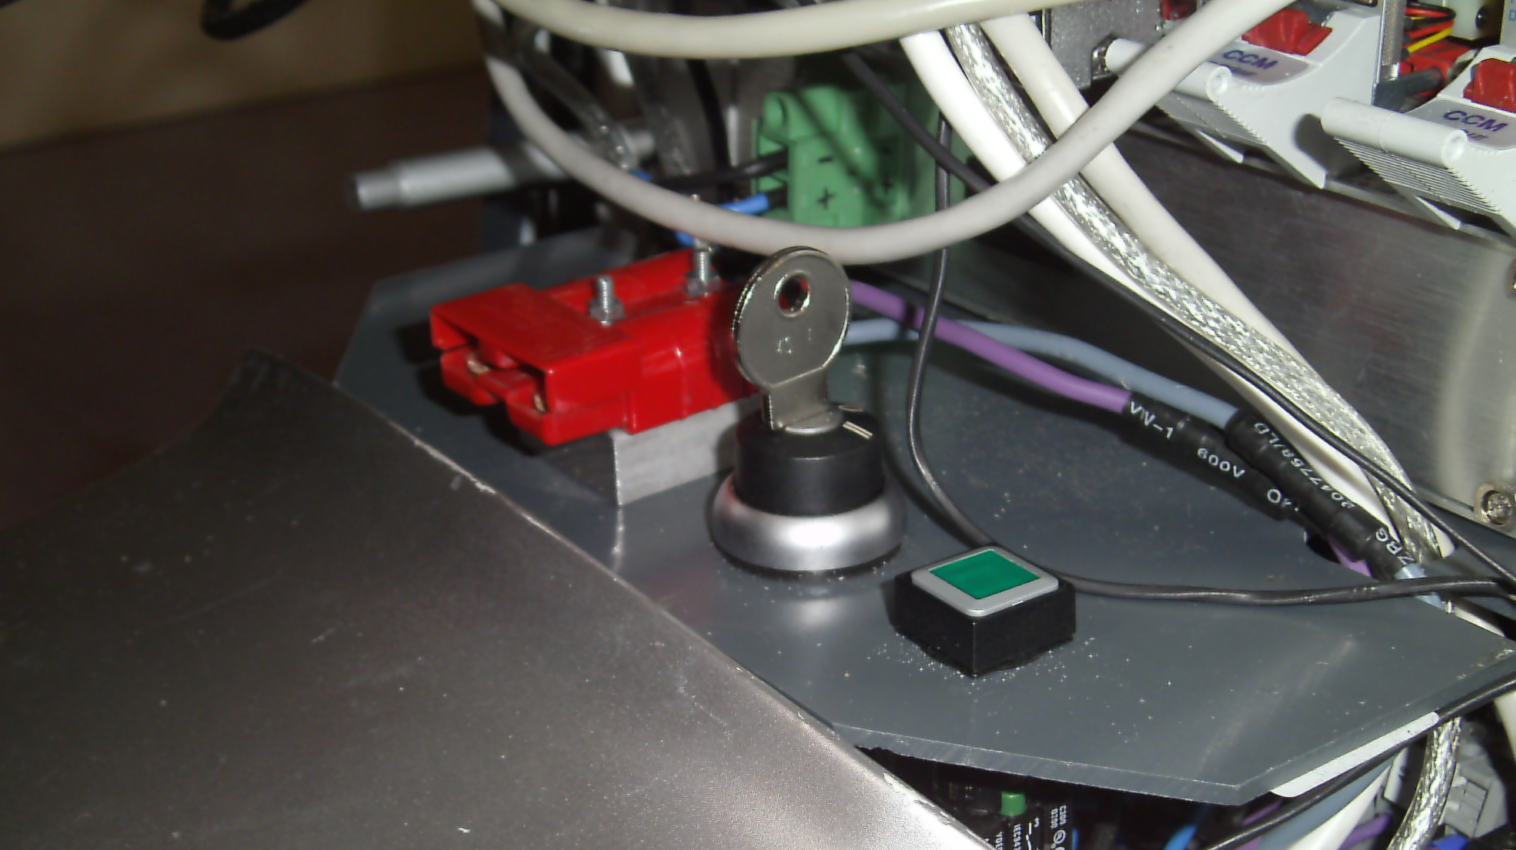
\includegraphics[width=0.3\textwidth]{images/key.png}
\end{center}


\subsection{Logging in to the robot pcs}
For logging in with a remote PC to the robot pcs you have to have an account on the robot. If you don't have an account contact your local robot administrator to create one for you (see the section \ref{sec:account}). Use ssh to login (in this example to pc1 of cob3-3)

\begin{lstlisting}
ssh -X user_name@cob3-3-pc1
\end{lstlisting}

\subsection{Bringup the robot}
\textbf{Note: The following steps can only be done once by one person at the same time. It is not possible to start for example mulitple roscore or brinup.}

The first step to bringup the robot is to start a roscore, this is necessary to have communication between the nodes. You can run it using
\begin{lstlisting}
roscore
\end{lstlisting}

If you want to run the robot you have a launch file for launching all the components of the robot. It is located in the package cob\_bringup.
\begin{lstlisting}
roslaunch cob_bringup robot.launch
\end{lstlisting}

Now all drivers and core components should be started so you can continue and have a look at the robot status in the dashboard or moving the robot using joystick or command\_gui.

\subsection{Using dashboard and command\_gui}
To know the state of all the components of the robot you can use the dashboard tool. To move the robot you can use the command\_gui. You can start both with
\begin{lstlisting}
roslaunch cob_bringup dashboard.launch
\end{lstlisting}

After launching this file you will see two GUIs on your screen: the smaller one is the dashboard, which gives you information about the current status of the robot and its components as well as the emergency stop status. The bigger one is called command\_gui and offers a wide range of buttons to move the robot to predefined positions using low level control commands. It also offers buttons for initialising and recovering the actuators. The emergency stop status is visible in the upper left corner of the command\_gui. Before initialising or moving the robot, check that the status is OK.

\subsubsection{cob\_dashboard}\label{subsec:dashboard}
The dashboard is an important tool where you can check the state of the robot, it is recommended that you have it always opened. The dashboard looks like this:

\begin{center}
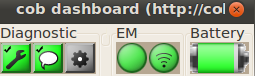
\includegraphics[width=0.55\textwidth]{images/dashboard.png}
\end{center}
If you click the first button, you will see a new window popping up with three levels: Errors, Warnings and All. There you can see the state of each component at any time. The status monitoring is divided into Actuators, Sensors and other. The other buttons are for showing diagnostics, motors, emergency status and battery state. In the case of the Care-O-bot we have disable the buttons for the Motors, you see them always in red.

\begin{center}
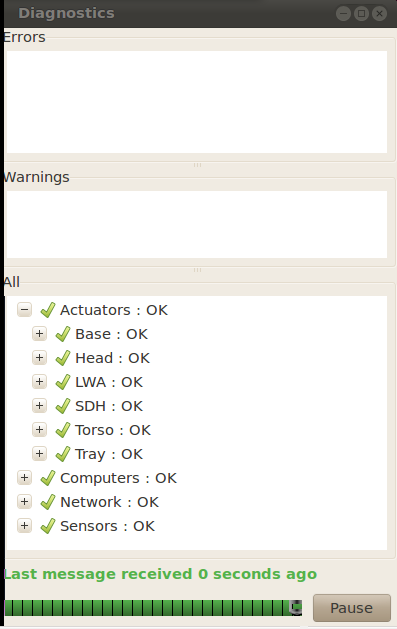
\includegraphics[width=0.45\textwidth]{images/diagnostics.png}
\end{center}

All diagnostics information for the actors and sensors should be green after successfully initializing the components, see section \ref{subsec:command_gui}.

\subsubsection{cob\_command\_gui}\label{subsec:command_gui}
The command gui can be used for sending low level movement commands to the robot components. The standard view of the command\_gui is:
\begin{center}
 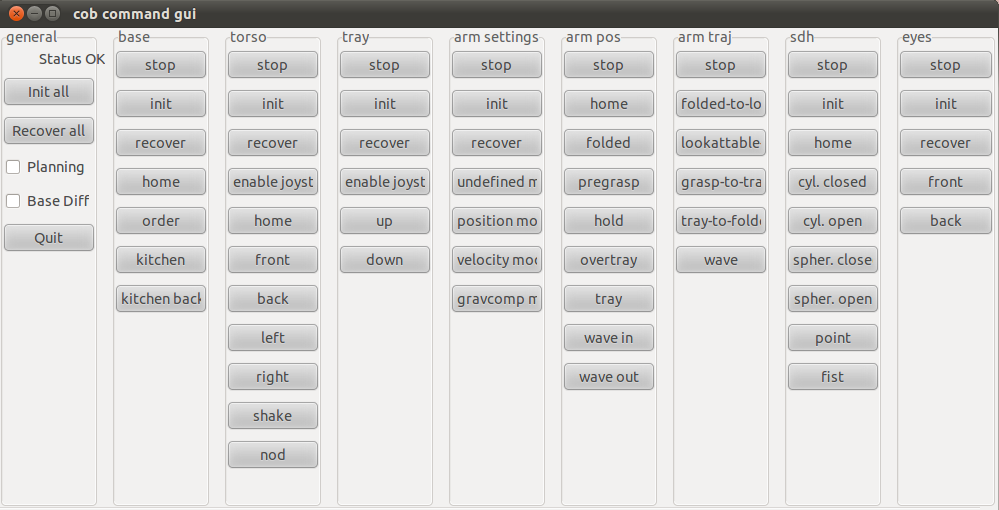
\includegraphics[width=1\textwidth]{images/cob_command_gui.png}
\end{center}

In this screen-shot you can see different columns: general, base, torso, tray, arm settings, arm pos, arm traj, sdh and eyes. The first column is very important, when you run the robot. If you want to move it, first initialize all components with a click on \texttt{init all} and make sure that the \textbf{emergency stop is not active}. It will take some time and the actuators will do their homing sequence if necessary. After an emergency stop was activated, each component has to be recovered. Therefore press the button \texttt{recover all}. 

The other columns of the components have different predefined positions where you can move to. Additionally Each component has a \texttt{stop}, \texttt{init} and \texttt{recover} button, to stop, initialize or recover a single component.

\subsection{Rviz}
RVIZ is a tool that visualizes data from the robot, e.g. the sensor data from the laser scanners, but also information about the coordinate systems and transformations or the images from the cameras. You can add your own items to RVIZ to visualize topics, see more information at \footnote{\url{http://www.ros.org/wiki/rviz}}.

RVIZ needs to be started on your local machine. To be able to visualize topics from the robot export your \texttt{ROS\_MASTER\_URI} to the robot
\begin{lstlisting}
export ROS_MASTER_URI=http://cob3-X-pc1:11311
rosrun rviz rviz
\end{lstlisting}

To use a predefined configuration for Care-O-bot start rviz with
\begin{lstlisting}
export ROS_MASTER_URI=http://cob3-X-pc1:11311
roslaunch cob_bringup rviz.launch
\end{lstlisting}

You will see a screen like this:
\begin {center}
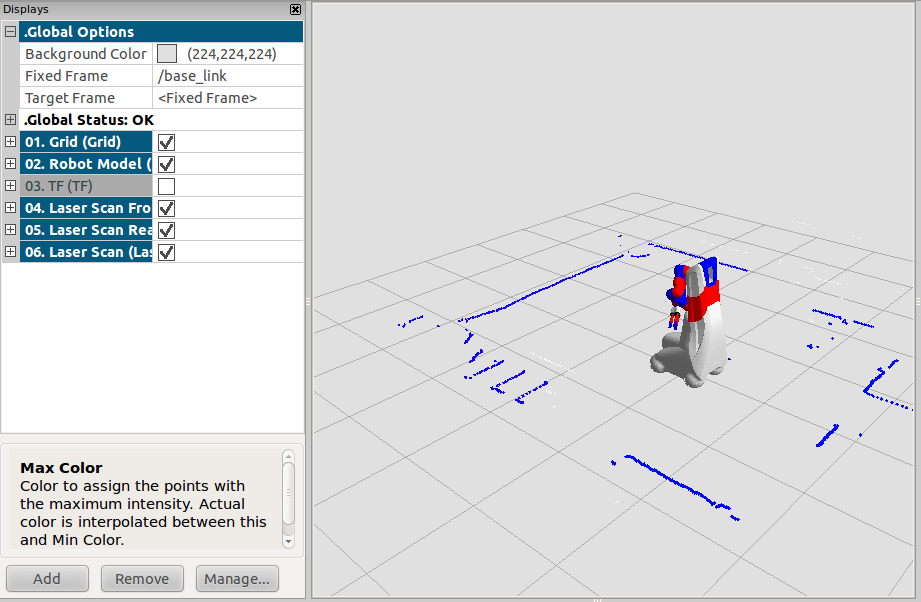
\includegraphics[width=1\textwidth]{images/rviz.png}
\end{center}

\subsection{Joystick}
To be able to use the joystick, initialize the components using the command\_gui. For moving the robot components, the dead-man\_button has to be pressed all the time, as soon as the button is released all hardware components will be stopped immediately. 

\begin{itemize}
\item For moving the base: Hold the dead-man button and use the base rotation and translation axis to move the base.
\item For moving the torso: Hold the dead-man button and the upper or lower neck button, then use the up\_down or left\_right axis to move the torso.
\item For moving the tray: Hold the dead-man button and the tray button, then use the up\_down axis to move the tray.
\item For moving the arm: Hold the dead-man button and one of the arm buttons, then use the up\_down or left\_right axis to move the selected arm joints.
\end{itemize}

Have a look at the following image to see which buttons command which components. 
\begin{center}
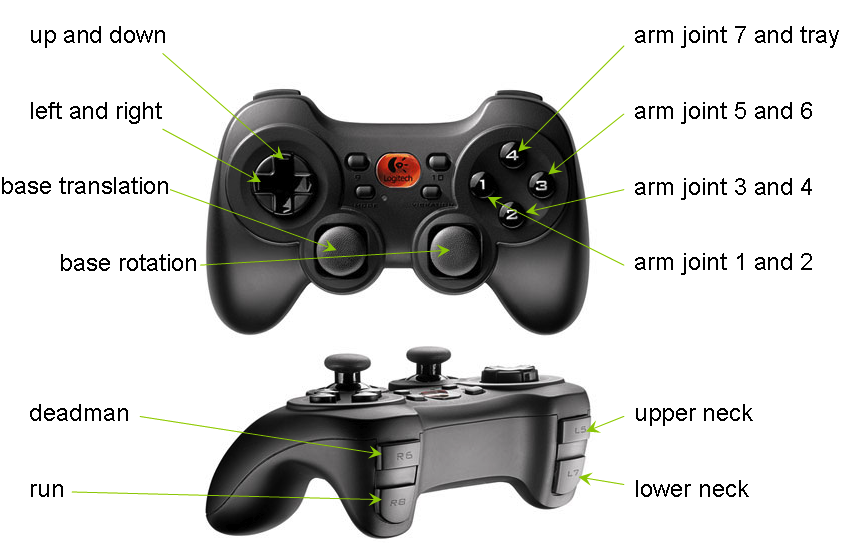
\includegraphics[width=1\textwidth]{images/joystick.png}
\end{center}

\section{Power down the robot}
To power down the robot press the emergency button and turn the key to position I, disconnect the power cable and turn off the power supply.

\section{Packing the robot}
tbd